\documentclass[fleqn]{article}
\usepackage{mathtools}
\usepackage{graphicx}
\usepackage{amssymb}
\usepackage[margin = 0.75in]{geometry}
\usepackage{enumerate}
\usepackage{color}
\usepackage{fancyvrb}
\usepackage{breqn}
\usepackage{fancyhdr}
\usepackage{multicol}
%\usepackage[latin1]{inputenc}
\usepackage{tikz}
\usepackage{circuitikz}
\usepackage{pgfplots}
\pgfplotsset{compat=1.8}

\usetikzlibrary{quotes,angles}

\pgfplotsset{vasymptote/.style={
    before end axis/.append code={
        \draw[densely dashed] ({rel axis cs:0,0} -| {axis cs:#1,0})
        -- ({rel axis cs:0,1} -| {axis cs:#1,0});
    }
}}

\renewcommand{\thispagestyle}[1]{}
\pagestyle{fancy}
\lhead{\textbf{NAME:}}
\rhead{}

\begin{document}
\title{Math 120R.002 Exam 4 Version A}
\author{Ammon Washburn}
\date{12.04.14}
\maketitle

\section*{Instructions:} 
Please show all of your work for each question. 
The point values for each question are located at the beginning of the question. 
Mark your answers by circling your answer in the test booklet, and in the answer sheet provided.

\vspace{1in} 

\begin{tabular}{|p{6.5in}|} 
\hline 
\noindent By signing my name below, I agree that I am following all rules and regulations set forth by the Code of Academic Integrity.  Furthermore, I agree that I am following all rules set by my instructor and by the course policy for this exam.  This includes ensuring that all calculator programs except possibly QUADRATIC FORMULA have been deleted.\\
\vspace{.3 in}\\
\underline{Signature:	\hspace{2.5 in}	Date:\hspace{1.25 in}}\\
\hline 
\end{tabular} 

\vspace{10pt}
\begin{center}
{\Large $\underline{\mathbf{Formulas}}$}
\end{center}
\begin{align*}
 \cos (2 \theta) & = \cos ^2 (\theta) - \sin ^2 (\theta) & \sin(2 \theta) & = 2 \sin(\theta)\cos(\theta) \\
 & = 2 \cos^2 (\theta) - 1 \\
 & = 1 - 2 \sin ^2 (\theta)\\
 \tan(2\theta) & = \frac{2\tan(\theta)}{1 - \tan^2(\theta)} \\
 \sin (x + y) & = \sin (x) \cos(y) + \cos (x) \sin (y) & \sin (x - y) & = \sin (x) \cos(y) - \cos (x) \sin (y)\\
 \cos (x + y) & = \cos (x) \cos (y) - \sin (x) \sin (y) & \cos (x - y) & = \cos (x) \cos (y) + \sin (x) \sin (y) \\
 \tan (x + y) & = \frac{\tan(x) + \tan(y)}{1 - \tan(x)\tan(y)} & \tan (x - y) & = \frac{\tan(x) - \tan(y)}{1 + \tan(x)\tan(y)} \\
\end{align*}


\pagebreak
\thispagestyle{fancy}{
\lhead{}
\rhead{/30}}

\begin{enumerate}
\section*{Free Response}
\item (20 points) Let sin($\theta) = \frac{1}{2}$ with $\theta$ in Quadrant I.  Let cot($\phi) = -\frac{4}{3}$ with $\phi$ in Quadrant II.  
\begin{enumerate}
\item Evaluate sin$(\theta + \phi)$.  Your answer should be exact. {\bf No decimals!}

\vspace{3.7in}

\item Evaluate $\cos(2\theta)$.  You answer should be exact. {\bf No decimals!}

\vspace{1.5in}
\end{enumerate}

\item (10 points) Prove the following trig identities using the basic identities.  Show each step.

\begin{enumerate}
\item $\cos(u)(\tan(u) + \cot(u)) = \csc(u)$
\vspace{1.5in}
\item $\cos(\theta) - \sec(\theta) = -\tan(\theta)$
\end{enumerate}
\vspace{0.5in}

\pagebreak
\thispagestyle{fancy}{
\lhead{}
\rhead{/20}}

\item (8 points) If cannon ball fired from a cannon at an initial velocity of 128 feet/second with an angle of elevation of $\theta$ then the maximum height it reaches is determined by

\begin{align*}
M(\theta) = \frac{128^2\sin^2(\theta)}{64}
\end{align*}

\begin{enumerate}
\item At what angle should the cannon be fired so that the maximum height of the cannon ball is 150 feet?
\vspace{2 in}
\item Is it possible for the cannon ball to reach a maximum height of 256 feet? Why or why not?
\vspace{1in}
\end{enumerate}

\begin{minipage}{0.6\textwidth}
\item
(12 points) The pilot of the plane $P$ measures the angle of depression to two different ships $A$ and $B$ as $40^\circ$ and $75^\circ$ respectively.
If the plane is flying at a height of $30,000$ feet, what is the distance between the two ships?

\end{minipage} \hspace{0.05\textwidth}
\begin{minipage}{0.2\textwidth}
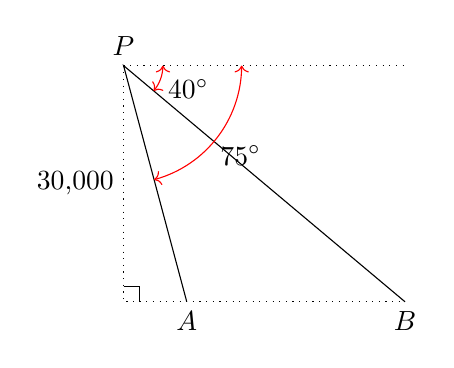
\begin{tikzpicture}
  \coordinate (t) at (3.575, 3);
  \coordinate (o) at (0, 0);
  \draw
    (0.803, 0) coordinate (a) node[below] {$A$}
    -- (0, 3) coordinate (p) node[above] {$P$}
    -- (3.575, 0) coordinate (b) node[below] {$B$}
    pic["$40^\circ$", draw=red, <->, angle eccentricity=1.75, angle radius=.5cm]
    {angle=b--p--t}
    pic["$75^\circ$", draw=red, <->, angle eccentricity=1.25, angle radius=1.5cm]
    {angle=a--p--t};
  \draw[dotted] (p) -- (o) node[midway, left] {30,000} -- (b);
  \draw[dotted] (p) -- (t);
  \draw (0, 0.2) -- (0.2, 0.2) -- (0.2, 0);
\end{tikzpicture}
\end{minipage}

\vspace{2 in}

\pagebreak
\thispagestyle{fancy}{
\lhead{}
\rhead{/20}}

\section*{Multiple Choice}

\item 
(5 points) A bicycle wheel with a diameter of 0.25 meters is traveling at a speed of 30 kmph.
What is the approximate angular speed of the tire, in \textbf{radians per second}? (Hint: 1000 meters = 1 kilometer)

\begin{enumerate}
\item $120 \; \frac{rad}{s}$

\item $60 \; \frac{rad}{s}$

\item $33.3 \; \frac{rad}{s}$

\item $16.6 \; \frac{rad}{s}$

\item None of the above

\end{enumerate}

\vspace{0.5in}

\item
(5 points) A wedge is cut from a flat circular wheel of cheese.
The wedge has a central angle of $30^\circ$.
If the wheel has a radius of 3 inches, what is the area of the wedge?

\begin{enumerate}
\item $135 \; in^2$

\item $90 \; in^2$

\item $0.75\pi \; in^2$

\item $0.5\pi \; in^2$

\item None of the above

\end{enumerate}

\vspace{0.5in}

\item (5 points) Write $\tan(\theta)$ in terms of $\cos(\theta)$ for $\theta$ in quadrant I.

\begin{enumerate}
\item $\displaystyle -\frac{\sqrt{1 - \cos^2(\theta)}}{\cos(\theta)}$
\vspace{.05in}
\item $\displaystyle -\frac{\cos(\theta)}{\sqrt{1 - \cos^2(\theta)}}$
\vspace{.05in}
\item $\displaystyle \frac{\sqrt{1 - \cos^2(\theta)}}{\cos(\theta)}$
\vspace{.05in}
\item $\displaystyle \frac{\cos(\theta)}{\sqrt{1 - \cos^2(\theta)}}$
\vspace{.05in}
\item None of the above

\end{enumerate}

\vspace{0.5in}

\item
(5 points) A 100 foot tall tree casts a shadow that is 20 feet long.
What is the approximate angle of elevation of the sun?

\begin{enumerate}
\item between $10^\circ$ and $20^\circ$

\item between $20^\circ$ and $30^\circ$

\item between $60^\circ$ and $70^\circ$

\item between $70^\circ$ and $80^\circ$

\item None of the above

\end{enumerate}

\vspace{0.5in}

\item
(5 points) Find the exact value of $\tan(\sin^{-1}(x))$.

\begin{enumerate}
\item $\displaystyle \frac{1}{\sqrt{1 - x^2}}$
\vspace{.1in}
\item $\displaystyle \frac{\sqrt{1 - x^2}}{x}$
\vspace{.1in}
\item $\displaystyle \frac{x}{\sqrt{1 - x^2}}$
\vspace{.1in}
\item $x\sqrt{1-x^2}$
\vspace{.1in}
\item None of the above

\end{enumerate}

\vspace{0.5in}

\item
(5 points) For what values of $\theta$ is the following equation true?
\begin{align*}
\sin^3(\theta)+\sin(\theta)\cos^2(\theta) = \sin(\theta)
\end{align*}

\begin{enumerate}
\item All values of $\theta$

\item Only some values of $\theta$

\item No values of $\theta$

\end{enumerate}

\vspace{0.5in}

\item 
(5 points) Rewrite the following equation in the form $f(t) = k\sin(t + \varphi)$.
\begin{align*}
f(t) &= \sqrt{3}\sin(t) - \cos(t)
\end{align*}

\begin{enumerate}
\item $1 < k < 3$, $-\frac{\pi}{3}\leq \theta \leq 0$

\item $1 < k < 3$, $0 \leq \theta \leq \frac{\pi}{3}$

\item $3 < k < 5$, $-\frac{\pi}{3} \leq \theta \leq 0$

\item $3 < k < 5$, $0 \leq \theta \leq \frac{\pi}{3}$

\item None of the above

\end{enumerate}

\vspace{0.5in}

\item
(5 points) Use the Addition-Subtraction formula to simplify the following: $\sin(\pi/5)\cos(\pi/10) + \cos(\pi/5)\sin(\pi/10)$

\begin{enumerate}
\item $\sin(\pi/15)$

\item $\cos(\pi/15)$

\item $\sin(\pi/10)$

\item $\cos(\pi/10)$

\item None of the above

\end{enumerate}

\pagebreak
\thispagestyle{fancy}{
\rfoot{/100}
\rhead{/10}}

\item
(5 points) Suppose an arc along a circle is subtended by an angle of $60^{\circ}$ where the circle has a radius of 5 inches.  What is the length of the arc?

\begin{enumerate}
\item 750 inches
\item 300 inches
\item $\frac{25\pi}{6}$ inches
\item $\frac{5\pi}{3}$ inches
\item None of the above
\end{enumerate}

\vspace{0.5in}

\item
(5 points) Suppose $\tan(\theta) = 1/B$, and the terminal side of $\theta$ is in quadrant II.
Find $\sec(\theta)$.

\begin{enumerate}
\item $\displaystyle \frac{B}{\sqrt{1+B^2}}$

\item $\displaystyle \sqrt{1+B^2}$

\item $\displaystyle -\frac{B}{\sqrt{1+B^2}}$

\item $\displaystyle -\frac{\sqrt{1+B^2}}{B}$

\item None of the above

\end{enumerate}

\vspace{0.5in}



\end{enumerate}

\end{document}